\section{Related work}
\label{related}
%https://arxiv.org/pdf/2304.08465.pdf
%https://arxiv.org/pdf/2305.16807.pdf
% https://arxiv.org/pdf/2212.04489.pdf
%(1) try adding two z and correlation, (2) try mu, mu_hat with 30 images

% One of the most fundamental challenges in generative models is to work on real images. The efforts are focused mainly on finding the random images that create the generated image as mentioned in Section~\ref{sec:intro} as well as on edit while maintaining the input content/identity. In this section, we present how other methods tackle these problems problem.

% We divide this section into two: applications that use the DDPM sampling and the ones that use DDIM sampling. 

\subsection{Inversion of diffusion models}
Editing a real image using diffusion models requires extracting the noise vectors that would generate that image when used within the generative process. %The DDPM sampling is stochastic, therefore, it is not trivial to invert this model.
The vast majority of diffusion-based editing works use the DDIM scheme, which is a deterministic mapping from a single noise map to a generated image~\cite{Hertz22,Mokady22,Narek22,Guillaume22,Bram22,Parmar23,Adham22}. The original DDIM paper~\cite{Song21} suggested an efficient approximate inversion for that scheme. This method incurs a small error at every diffusion timestep, and these errors often accumulate into meaningful deviations when using classifier-free guidance~\cite{Ho21}. Mokady \etal~\cite{Mokady22} improve the reconstruction quality by fixing each timestep drifting. Their two-step approach first uses DDIM inversion to compute a sequence of noise vectors, and then uses this sequence to optimize the input null-text embedding at every timestep. Miyake \etal~\cite{miyake23}
achieve similar reconstruction accuracy through forward propagation without optimization, thereby enabling much faster editing processes. An improvement in the reconstruction quality was suggested by Han \etal~\cite{Han23} that integrate a regularization term into the null-text embedding optimization. % Proximal guidance was introduced by  
EDICT~\cite{Bram22} enables mathematically exact DDIM-inversion of real images by maintaining two coupled noise vectors which are used to invert each other in an alternating fashion. This method doubles the computation time of the diffusion process. %and cannot produce multiple results.
CycleDiffusion~\cite{Wu22} presents a DDPM-inversion method by recovering a sequence of noise vectors that perfectly reconstruct the image within the DDPM sampling process. As opposed to our method, their extracted noise maps are distributed like the native noise space of DDPM, which results in limited editing capabilities (see Figs.~\ref{fig:generated_vs_us},\ref{fig:cyclediffusion_vs_us}).

%\inbar{Direct Inversion: Optimization-Free Text-Driven Real Image Editing with Diffusion Models~\cite{Adham22}. Not sure we should cite them} \tomer{Cite them at the beginning of the paragraph where I left a comment (in addition to many other papers that use DDIM inversion)}

% edit a real image while keeping it as faithful as possible to the real content (structure/identity).

\subsection{Image editing using diffusion models}
% DDPM - interpolation+SDEdit
The DDPM sampling method is not popular for editing of real images. When used, it is typically done without exact inversion. %Ho et al.~\cite{Ho20} and Meng et al.~\cite{Meng22} edit images without inversion. 
Two examples are Ho \etal~\cite{Ho20}, who interpolate between real images, and Meng \etal~\cite{Meng22} who edit real images via user sketches or strokes (SDEdit). Both construct a noisy version of the real image and apply a backward diffusion after editing. They suffer from an inherent tradeoff between the realism of the generated image and its faithfulness to the original contents. %The balance between the two is controlled by the variance of the noise added to the image. 
DiffuseIT~\cite{Gihyun22} performs image translation guided by a reference image or by text, also without explicit inversion. They guide the generation process by losses that measure similarity to the original image~\cite{Prafulla21}.

% Text driven
A series of papers apply text-driven image-to-image translation using DDIM inversion. Narek \etal~\cite{Narek22} and Cao \etal~\cite{cao23} achieve this by manipulating spatial features and their self-attention inside the model during the diffusion process. Hertz \etal~\cite{Hertz22} change the attention maps of the original image according to the target text prompt and inject them into the diffusion process. DiffEdit~\cite{Guillaume22} automatically generates a mask for the regions of the image that need to be edited, based on source and target text prompts. This is used to enforce the faithfulness of the unedited regions to the original image, in order to battle the poor reconstruction quality obtained from the inversion. This method fails to predict accurate masks for complex prompts.%and/or very different from one another. 

% optimization methods
Some methods utilize model optimization based on the target text prompt.  DiffusionCLIP \cite{Kim22} uses model fine-tuning based on a CLIP loss with a target text. Imagic \cite{Bahjat22} first optimizes the target text embedding, and then optimizes the model to reconstruct the image with the optimized text embedding. %In the last part, they freeze the embedding and the model and use the diffusion process with text interpolation between the optimized one and the target one. 
UniTune~\cite{Valevski22} also uses fine-tuning and shows great success in making global stylistic changes and complex local edits while maintaining image structure. Other works like Palette~\cite{Saharia21} and InstructPix2Pix~\cite{Brooks22}, learn conditional diffusion models tailored for specific editing tasks. %The high computational cost of fine-tuning a diffusion model for a task or over an input image, however, makes it impractical as an interactive image editing tool. %Since our method is training-free, we do not view them as competitive algorithms.


\begin{figure}
%\vskip 0.2in
% \begin{center}
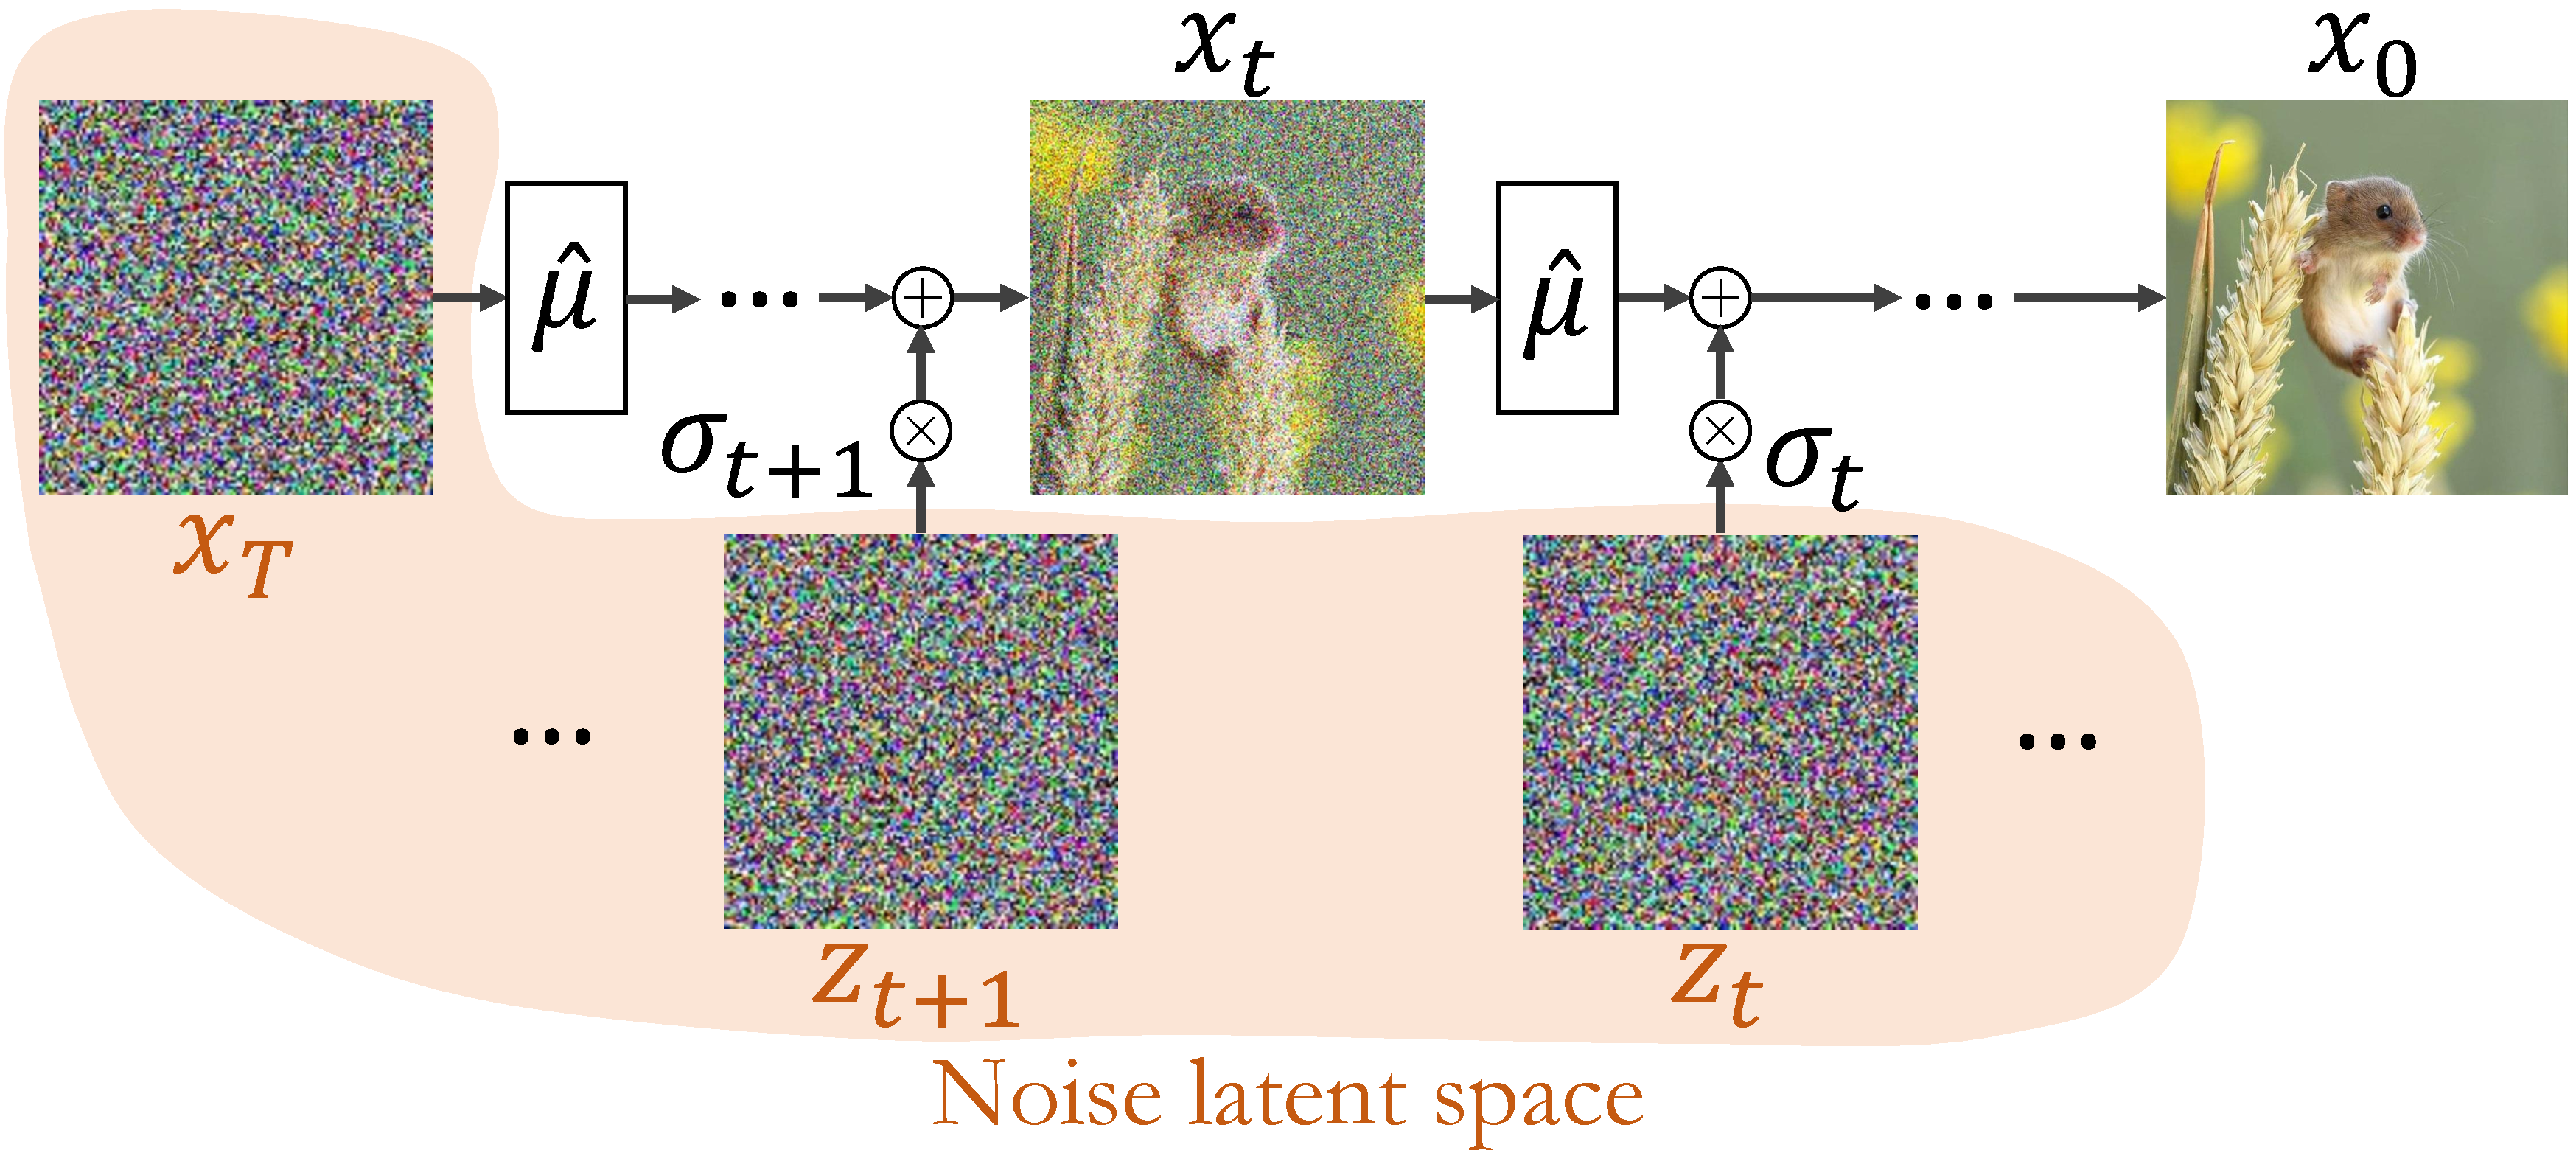
\includegraphics[width=\columnwidth]{ICCV23_submission/figures/DDPM_sampling_process.pdf}
\caption{\textbf{The DDPM latent noise space.} In DDPM, the generative (reverse) diffusion process synthesizes an image $x_0$ in $T$ steps, by utilizing $T+1$ noise maps, $\{x_T,z_T,\ldots,z_1\}$. We regard those noise maps as the latent code associated with the generated image.}
\label{fig:unfold}
% \end{center}
%\vskip -0.2in
\end{figure}


% The applications of inpaiting~\cite{Lugmayr22} and local edit via text ~\cite{avrahami22}, change only the pixels inside a pre-defined mask. Therefore, the content of the pixels outside the mask remains unaffected and they achieve both meaningful editing and background preservation. In these cases, a mask must be provided as input to tell the diffusion model what parts of the image should be edited. 


%\inbar{add Dall-E-2 - also editing}

% DDIM papers + inversion:
% - DiffusionCLIP

% DDIM papers + mask:
% - DIFFEDIT: DIFFUSION-BASED SEMANTIC IMAGE EDITING WITH MASK GUIDANCE
% DDIM papers + optimization:
% - Imagic (read about TEdBench)
% - DiffusionCLIP
% - Diffusion Autoencoders - should add?

% Not real images:
% - ILVR: Conditioning Method for Denoising Diffusion Probabilistic Models. Guided generating using a reference image- should add?
%\inbar{
%- GLIDE?
%- concurrent work: Zero-shot Image-to-Image Translation, MagicMix, FlexIt, DreamBooth, Eliminating Prior Bias for Semantic Image Editing
%via Dual-Cycle Diffusion, Asyrp?
%}

% Also, as the Prompt-to-Prompt technique
% requires fixing the attention weights, it is restricted to localized edits, and supports only a limited set
% of edit operations (adding or changing a word). Our method is inspired by Prompt-to-Prompt, and
% relaxes those restrictions.

